\documentclass[11pt,twoside]{article}
\usepackage{geometry}
\usepackage{enumerate}
\usepackage{latexsym,booktabs}
\usepackage{amsmath,amssymb}
\usepackage{graphicx}
\usepackage{natbib}
\usepackage{hyperref}
\usepackage[singlespacing]{setspace}

\geometry{a4paper,left=3cm,right=2.0cm, top=2cm, bottom=2.0cm}

\newtheorem{Definition}{Definition}
\newtheorem{Theorem}{Theorem}
\newtheorem{Lemma}{Lemma}
\newtheorem{Corollary}{Corollary}
\newtheorem{Proposition}{Proposition}
\newtheorem{Algorithm}{Algorithm}
\numberwithin{Theorem}{section}
\numberwithin{Definition}{section}
\numberwithin{Lemma}{section}
\numberwithin{Algorithm}{section}
\numberwithin{equation}{section}


\begin{document}

\pagestyle{empty}

% =============================================================================
% Title page
% =============================================================================
\begin{titlepage}
\vspace*{.5em}
\center
\vspace*{1em}
\vspace{2em}
\textbf{\Huge{Scotland Water - Lead Piping Data Cleaning}}\\[2em]
\textbf{\LARGE{by}}\\
\vspace{2em}
\textbf{\LARGE{Student name:}}\\
\vspace{1em}
\textbf{\LARGE{Student ID:}}\\
\vspace{6.5em}
\vspace{6.5em}
\Large{June 2020}\\
\vspace{3em}
\vfill
\end{titlepage}

\clearpage

% =============================================================================
% Acknowledgments, and own work declaration
% =============================================================================

% \begin{center}
% \Large{Acknowledgments}
% \end{center}

% Here come your acknowledgments ...

% \clearpage

\begin{center}
\Large{Own Work Declaration}
\end{center}
I declare that this my own work, and that no body has collborated, assisted
me on this work or any process related to this work.

\cleardoublepage



% =============================================================================
% Table of contents, tables, and pictures (if applicable)
% =============================================================================

\tableofcontents
\clearpage

\pagestyle{plain}
\setcounter{page}{1}
\pagenumbering{Roman}

\cleardoublepage

\pagenumbering{arabic}
\setcounter{page}{1}


\clearpage

\section*{Executive summary}
\label{sec.summary}
In this project, we check the lead polution condtion of water pipes in the region of Scottish Water company in Scotlan. To do this, we stripped nine data sets out of nine tables for us to use. Some of information from them are useful, however, other are not. We built a data feature dictionary to find the connections between them and extract useful information. For example, we find the information about the age, price of the area house, and whether houses' communication water pipe have been updated. Also, the information collected by the Scottish Water company is deconstructed and summarized by the data sets we genearted. The information we find include whether the regional water quality is polluted by lead over limit and treatment effect as well as various physical parameters of water and so on. By summarizing and analyzing these basic data information, we have generated some new data for studying the level of lead pollution in water supply pipelines in this area.

\clearpage

\section{Introduction}
\label{sec.intro}
Lead is one of the most important environmental pollutants and has been shown in several studies to be a trigger for health problems according to \cite{ei}. This is because lead poisoning can occur when the lead enters the body. Small amounts of lead can accumulate over time and cause health problems. The health effects of lead poisoning cannot be ignored. Exposure to lead can be harmful, especially to unborn babies and young children who absorb more lead as their bones develop. Signs and symptoms of young children can include irritability and fatigue, loss of appetite and weight loss, abdominal pain, vomiting, and constipation according to \cite{stacy}. In addition, exposure to lead from drinking contaminated water can cause illness in adults. High blood pressure, abdominal pain, constipation, joint and muscle pain, and headache are suspicious symptoms in adults (Scottish government \citeyear{government}).

In modern life, the risk of human lead poisoning is very low because lead is now generally not used in paint, petrol, or food containers. As a result, most people have very little exposure to lead (WHO, \citeyear{who}). However, one of the main potential risks may be drinking tap water. People need to be especially careful if the property has lead pipes, water tanks, or pipes with lead fittings, as this can lead to a polluted water supply according to \cite{tee}. And this problem is taken seriously by the Scotland government. The government stipulated that all drinking water should meet the tighter standard for lead (10$\mu$g/l) that came into force in December 2013 (Scotland Government, \citeyear{government}). Although most modern water pipes are made of lead-free materials, however, houses built before 1970 may have a water pipe that connects the property to the water main in the street that contains lead. Hence, it is the strategic goal of the Scottish Water company to replace this part of the water supply pipeline and ensure the water quality of customers. And the goal of the company is to increase the reliability, resilience, and sustainability of its services to realize lead-free water supply. Hence, the Scottish Water company is striving to achieve two points for its customers: 1. At least one tap in the property is supplied with water that has not been in contact with lead pipes. 2. The level of lead in the water is no higher than 3 $\mu$g/l.

\clearpage

\section{Background}
\label{sec:background}
The World Health Organization advises that there is no safe level of lead and the current EU Drinking Water Directive allows a maximum level of 10 $\mu$g/l (European Union Scientific Committees, \citeyear{european}). However, the EU Drinking Water is being revised, with lead levels proposed to reduce to 5 $\mu$g/l according to \cite{aquatech}. Hence, the regulatory sampling will be targeted at high-risk areas, including the areas of Scottish Water (\cite{sw}). So, compliance with Scottish Water will drop. However, standards recognize achieving zero lead is unachievable as many brass plumbing fittings are extremely secretive and numerous which contain small amounts of lead.
Scottish Water company has made many efforts and achieved certain results before this. The following is a summary of the information available from Scottish Water company in their treatment of lead pollution in water.
Starting with regulations, the company takes steps to meet the standards. Phosphate is added to water to reduce plumbosolvency at 85 WTW. The phosphate reacts with lead pipes to form a chemical layer which reduces the dissolution of lead into the drinking water. The amount of phosphate has been optimized for each zone to obtain lowest lead level at the minimum possible dose based on performance of lead test rigs. The majority of phosphate dosing equipment was installed between 1996 and 2006 in response to the lead standards of 50$\mu$g/l to 25$\mu$g/l. The measures taken by the company are effective (Drinking Water Quality Division, \citeyear{drinking}). The 2012 Statistical survey indicated that on average 4\% of the 1.8 million communications pipes were lead (72,000) (90\% confidence level and + 10\% accuracy). The levels varied by zone from 0\% to 37\%. And the surveys of customer incoming supply pipe indicated a similar percentage of lead but not always aligned. Also, communications pipes can supply multiple properties (2.6 million properties). The random, statistical, regulatory sampling from all property ages indicates that:

\begin{enumerate}
\item over 97\% of samples had lead levels less than 5 $\mu$g/l.
\item 1.5\% of samples were between 5 and 10 $\mu$g/l (27,000 connections).
\item 1.0\% of samples were over 10 $\mu$g/l (18,000 connections).
\end{enumerate}

However, it is not enough to meet the latest regulatory standards. There are two reasons.
For Scottish Water company, the lead is due to contamination by the pipe network and plumbing, the main causes are: 1. The chemical layer can quickly destabilize with changes in available phosphate in the water. 2. Forming the layer on old pipes can take much longer than new pipes (as used in test rigs) due to their condition. 3. Performance may be harder to achieve with soft organic laden waters. 4. The raw materials for phosphate are finite and used by other industries.

For customers, it is because of less awareness of lead from customers and the plumbing in their home: 1. Most of SW’s customers believe that there are no/very few lead pipes still present in the system. 2. Under 30’s has little awareness of lead in the environment. 3. Lead pipes are a ‘forgotten subject’ little about it in the trade press. 4. The supply pipes, plumbing \& storage tanks, solder \& joints and brass fittings which contains lead can be used by customers (Scottish Water, \citeyear{sw2}).
In conclusion, the places where Scottish Water company need to improve and communicates with customers are: 1. Lead communications (Scottish Water) and or supply pipes (Customer). 2. Lead plumbing \& storage tanks (Customer). 3. Lead solder \& joints (Both). 4. Brass fittings (Both).

To this end, Scottish Water company has prepared the following plan to further reduce the level of lead pollution in the water. 1. Increasing the knowledge of the levels and location of lead within the water supply system through increased sampling. 2. Informing customers about lead in drinking water – raising awareness \& helping them to reduce their risk of exposure. 3. Optimizing phosphate dosing – seeking to achieve the lowest levels of lead in drinking water possible at customers taps, until lead pipe removal allows dosing to be stopped. 4. Remove lead pipes from the public network – using reactive and planned programs to minimize risk and support the switch off of phosphate dosing. 5. Ensuring customer pipes in contact with drinking water are removed - work with customers and stakeholders to encourage improvements to their supply pipes and plumbing to ensure they have access to lead free drinking water.

\clearpage

\section{Exploratory \& initial data analysis}
\label{sec.explore}

\subsection{Raw data}
\label{sec:raw}
When exploring the dataset, the first question that needs to be concerned is where does the data come from? The sources of data are mainly divided into three categories according to their uses, which are respectively: 1. Data sets related to the identification of lead concentrations in local water pipes. 2. Data sets related to the identification of phosphates in local water pipes to reduce lead concentrations. 3. Collect data sets of user information, street information, and a series of public facilities information within the scope of Scottish Water. The following is a brief description of the source and functionality of each dataset by category.

\begin{enumerate}

\item Datasets related to the identification of lead concentrations in local water pipes.

SW - Lead Comm Pipe Replacements (2004-2018).csv. This dataset contains information about the completeness status of the communication pipes for each street postcode. For feature ‘Wo Create Date’ it records the date of replacing the lead Comm Pipe. For feature ‘Wo Completed Status’ it records the outcome of the working status of replacing lead pipes. For feature ‘Street postcode’ it records the street postcode which the lead Communication pipe belongs to. For feature ‘Ads Water Operational Area’ it records the address of the water operation area. For feature ‘Ads Water Supply Zone’ it records the address of the water supply zone.

SW - Comm pipe data.xls. This dataset contains the detailed information of the communication pipes of the Scottish Water company. For the feature ‘Street postcode’ it records the street postcode which the lead Communication pipe belongs to. For the feature ‘AR10\_PROPERTYID’ it records the unique representation of each property. For the feature ‘Property Type’ it records the type of property serviced by communication pipe. For the feature ‘Is the property age pre-1970?’ it records whether the property age is before 1970. For the feature ‘Pipe Material’ it records the type of material which the communication pipe is made of as at the date of inspection. For the feature ‘Date’ it records the date of pipe inspection.

\item Datasets related to the identification of phosphates in local water pipes to reduce lead concentrations.

SW - Scottish Water Zonal Phosphate Levels.xls. This dataset contains descriptive data on how the release of phosphate adapts environments in various WOA regions. For feature ‘Sample Date’, it records the date of sampling. For feature ‘Hydrogen ion’, it records the amount of hydrogen ion dosing in drinking water at Water Treatment Zone. For feature ‘Lead’, it records the amount of lead dosing in drinking water at Water Treatment Zone. For feature ‘Phosphorus’, it records the amount of orthophosphate dosing in drinking water at Water Treatment Zone. For feature ‘Temperature’, it records the ‘Temperature at Water Treatment Zone’. For feature ‘Rig’, it records the information of the WOA name.

SW - Phosphate Dosing WTWs Y or N.xlsx. This dataset describes the information on whether or not orthophosphate dosing of drinking water occurs in the water treatment zone. The feature ‘WTW Name (Code)’ can be used as a connect column of this dataset with the dataset ‘SW - All Lead WQ Samples (2010-18).xls’. Its meaning is the name of the Water Treatment Zone and it is the same as the meaning of Water Treatment Area Name in dataset ‘SW - All Lead WQ Samples (2010-18).xls’. The feature ‘Phosphate Dosing on Site?’ records whether or not orthophosphate dosing of drinking water occurs in the water treatment zone.

SW - All Lead WQ Samples (2010-18).xls. This dataset mainly contains the water quality detection information of the lead poisoning in the area of Scottish Water company. For the feature ‘Sample Date Timestamp’ it records the sample collection date and time. For the feature ‘Result Numeric Entry’ it records the lead concentration in tap water (in $\mu$g/l). For the feature ‘DMA Name and ID’ it records the District Meter Area Name and ID. For the feature ‘RSZ Name and ID’ it records the Regulatory Supply Zone Name and ID. For the feature ‘RSZ Water System Name and Id’ it records the Water Treatment Area Name and Id. For the feature ‘Sample Date’ it records the Sample collection date. For the feature ‘Street Postcode’ it records the Street Postcode. For the feature ‘WOA Name and Id’ it records the name and id of water Operational Area. For the feature ‘WSZ Name and Id’ it records the name and id of Water Supply Zone.

\item Collect datasets of user information, street information and a series of public facilities information within the scope of Scottish Water.

Other - UK-HPI-full-file-2019-03.csv. This dataset is about the UK House Price Index (UK HPI) that captures changes in the value of residential properties. The UK HPI uses sales data collected on residential housing transactions, whether for cash or with a mortgage. Properties have been included: in England and Wales since January 1995 in Scotland since January 2004 in Northern Ireland since January 2005. Data is available at a national and regional level, as well as counties, local authorities, and London boroughs. In this dataset, the useful features are ‘Date’, ‘RegionName’, ‘CouncilArea2018Code’, and ‘average price’. For the ‘Date’, it records every sample’s time. The period of each ‘Date’ sample is per month. For ‘RegionName’, it records each name of the selected region. The target region of Scottish Water is contained by some of the region names. And we only need to select them out when merging. For ‘CouncilArea2018Code’, it is an individual identifier of each ‘RegionName’. The usage of it is to merge this dataset by this column with the same column in the dataset ‘Other - Postcode\_ household count\_ urban class.csv’. For ‘average price’, it records the average house price in the region on each date in a monthly period.

Other - SAA\_PropertyAgeData.csv. This dataset is about the UK property year recording. The features are ‘UPRN’, ‘Postcode’, ‘Building\_Type’, ‘Age\_Year’, ‘Age\_Category’, ‘XCOORD’, ‘YCOORD’. For ‘UPRN’, it stands for Unique Property Reference Number and was created by the Ordnance Survey (OS) from the local UK government. It consists of numbers of up to 12 digits in length and it has a unique number for each land or property. For ‘Postcode’, it is the street postcode which can be used to merge with other datasets. For ‘Building\_Type’, it records the type of the property. This feature might be a useful predictor with \% of the detached buildings in a postcode count potentially. For ‘Age\_Year’ and ‘Age\_Category’, they record the year of the house built. It should be noted that these two columns of data are not a complete integer type, and other descriptive data need to be classified manually. For ‘XCOORD’ and ‘YCOORD’, they are the coordinates from the Digimap projection system.

Other - Postcode\_ household count\_ urban class.csv. This dataset is about the Scottish Government Urban Rural Classification’s information for each street postcode we have in the region of Scottish Water. The useful features in this dataset are ‘Street postcode’, ‘CouncilArea2018Code’, ‘CensusHouseholdCount2011’ and ‘CensusPopulationCount2011’. For ‘Street postcode’ and ‘CouncilArea2018Code’, the usage of them are to merge this dataset by this column with the same column in the dataset we introduced above. For ‘CensusHouseholdCount2011’ and ‘CensusPopulationCount2011’ they record the number of households and population in each street postcode based on Scottish 2011 census.

SW - Postcodes linked to SW Zonal Structure.xlsb. This dataset is an association table that connects the street code with its corresponding WOA, RSZ, WSZ, and DMA region. For features with ‘WOA’, they record the ID and name of each Water Operational Area connecting with the postcode. For features with ‘RSZ’, it records the ID and name of each Regulatory Supply Zone connecting with the postcode. For features with ‘WSZ’, it records the ID and name of each Water Supply Zone connecting with the postcode. features with ‘DMA’, it records the ID and name of each District Meter Area connecting with the postcode. Also, the feature ‘Total properties’ records the number of properties in each DMA, and the feature ‘Count’ records the number of DMA in each postcode.

\end{enumerate}

\clearpage

\subsection{Explorotary data analysis}
For the dataset generated from ‘SW - Scottish Water Zonal Phosphate Levels.xls’, it is very hard to use. First, it is not a relational dataset, so it is hard to directly merge it with other datasets in the use of the Water Operational Area (WOA) name or other identification letters. Second, the dataset is detached, which means the dataset is separated by the different areas with orientation south, east, west, and north. Third, the separate part of the dataset has the WOA name recorded hazily, which means the name of each street cannot exactly match the street names in the other datasets. So, in this dataset, first, the name of each WOA should be extracted by region and the key part of the string subtracted from the name should be intercepted for a fuzzy search. To do this, we do not need the region separation so we combine the geographical WOA names of each region into a single column to make it become a relational dataset that can be correlated (Pandas: ignore\_index = True). Second, we find the WOA name by converting each WOA name to a string and do slicing according to certain rules. The example format of each WOA name is ‘XX - Lead rig – WOA name (alias) Zone (name of Pumping Station)’. We should only use the WOA name and slice this part as our merging part. In this procedure, we find that the signs ‘/’, ‘A, B, C’, ‘()’ are too detailed and do not have these characters in another associated table. So, we ignore those signs in the WOA name merge. We find there are only 99 WOA in the whole region of Scottish Water company. We find the feature ‘Total organic carbon’ and ‘Optimization status change’ has too little data and they are meaningless in the research, so we directly delete them and do not obtain them in the merged dataset. Also, the feature ‘Sample Comments’ is tanglesome. We view this feature one by one and find it is not reasonable, so we drop it from the merged dataset. Another problem we find is the WOA name in ‘SW - Postcodes linked to SW Zonal Structure.xlsb’ we are merging for is overrated. Some of the WOA name in the ‘SW - Scottish Water Zonal Phosphate Levels.xls’ dataset has several small subdivisions. In this case, we calculate the mean value of each overrated value matching to the subdivision part. After screening, we also found that some sample points of data were noise points (as shown in the figure below) and some sample points were missing due to too late screening time to enter data (as shown in the figure below). In the case of noise point, we use the method of moving average to detect and delete the noise points. We choose 5 days sample points before each sample points data to calculate the moving average and delete the points are over 20 times than the moving average. In the case of missing value, we directly remove the data points since we need to use the average value of the last 5 points, and the missing points are not indispensable.

Note that we use median instead of average value to judge whether a data point collected by rig is an abnormal value, which is because that median is a much more robust value compared to moving average. By experiment, we see that the moving average is greatly affected by the extreme values, and could misclassify some of the normal values as abnormal since the moving average is pulled away by the extreme value from normal values.

\begin{figure}[!ht]
    \centering
    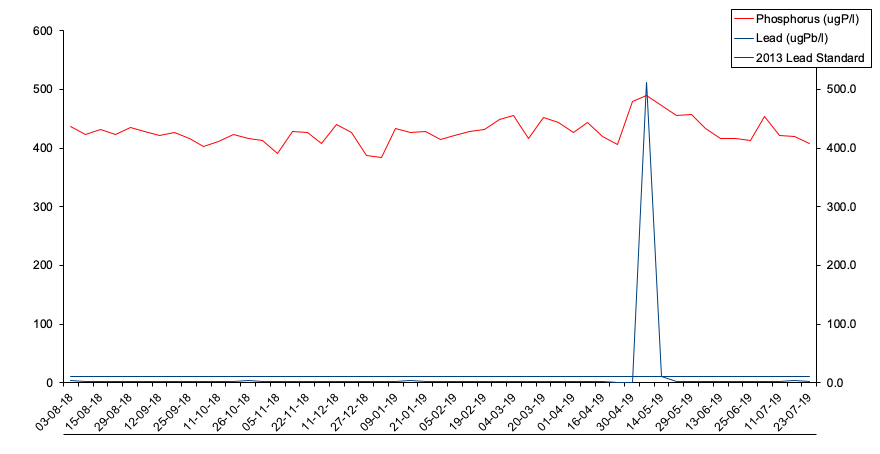
\includegraphics[width=0.8\textwidth]{p1.png}
    \caption{Example 1 of extreme values}
    \end{figure}

\begin{figure}[!ht]
    \centering
    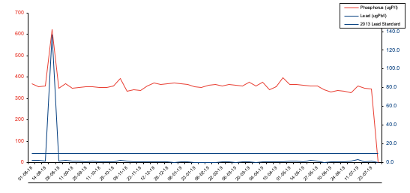
\includegraphics[width=0.8\textwidth]{p2.png}
    \caption{Example 2 of extreme values}
    \end{figure}

Below are examples showing what kind of sample points (in blue) we have deleted from the dataset.

\begin{figure}[!ht]
    \centering
    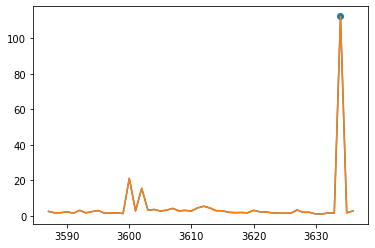
\includegraphics[width=0.45\textwidth]{p4.png}
    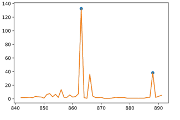
\includegraphics[width=0.45\textwidth]{p5.png}\\
    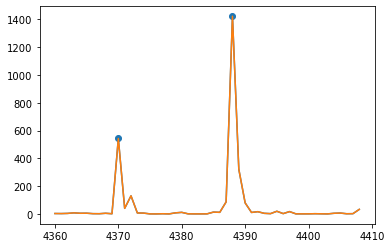
\includegraphics[width=0.45\textwidth]{p6.png}
    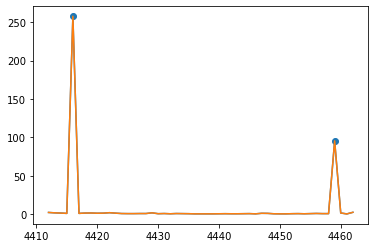
\includegraphics[width=0.45\textwidth]{p7.png}
    \caption{Extreme values marked by our algorithm}
    \end{figure}

Now the result of doing the above things is one WOA matches one sensor. Then, we need to search the tables for WOA and WSZ at the same time by extracting the keywords contains the original WOA name is the dataset ‘SW - Scottish Water Zonal Phosphate Levels.xls’. we then associate the searched keywords with the postcode. Hence, such a sensor corresponds to a lot of Postcodes. The existing values collected for each sensor's associated physical coefficients are the average of the last five non-null values. We then do a reverse search to find which sensors correspond to which Postcodes and calculate the average of the physical parameters of all sensors based on each Postcode. These include: ‘Hydrogen ion’, ‘Lead concentration’, ‘Phosphorus’ and ‘Temperature’.

For the dataset generated from ‘Other - UK-HPI-full-file-2019-03.csv’, after we do the initial data analysis work, we make sure that all the average price is for 411 areas region and each of them has the last date price collection at 01/03/2019. Also, each region has at least a one-year collection of samples for data sampling for each month period. Hence, we could make use of the last year's period, that is, the 12-months’ data sample of each region to find an average region house price of each region in an average year count. After making sure the dataset is as expected as it described, we calculate the average region house price of each area in an average year count. Below is a frequency distribution histogram of the house prices in the region of Scottish Water company. We find that most of the houses are priced between £200,000 and £400,000.

\begin{figure}[!ht]
    \centering
    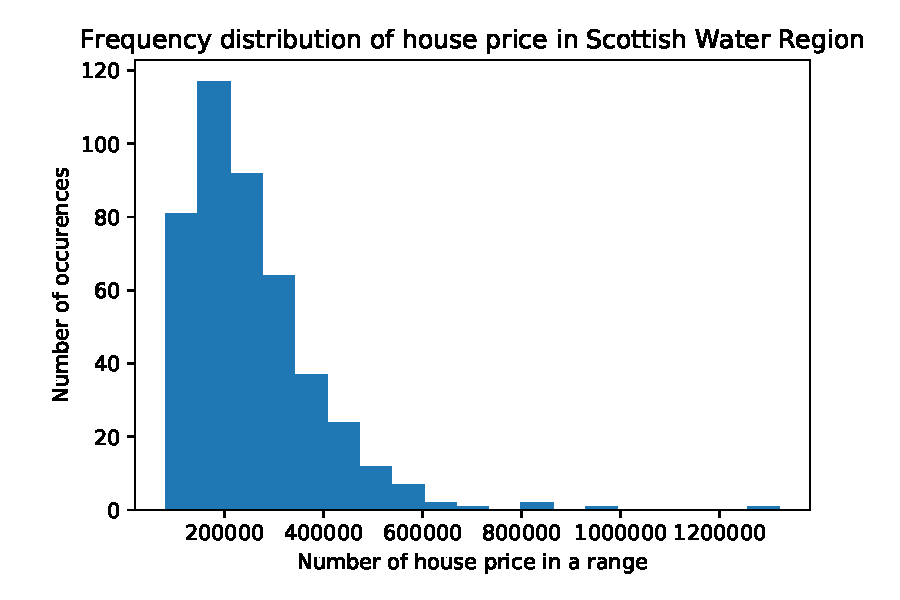
\includegraphics[width=0.6\textwidth]{p8.pdf}
    \end{figure}

However, we are still not finished. The final goal of this dataset is to calculate the average price base on the distinguishing identifier in the level of the street postcode. Hence, we need to read in another dataset which can be used to connect the two datasets with the same feature. After checking at the features dictionary, we find both of the dataset ‘Other - Postcode\_ household count\_ urban class.csv’ and ‘Other - UK-HPI-full-file-2019-03.csv’ contains the feature ‘CouncilArea2018Code’ and the ‘Other - Postcode\_ household count\_ urban class.csv’ contains the feature ‘Street postcode’. Hence, we read in the ‘Other - Postcode\_ household count\_ urban class.csv’ contains the feature ‘Street postcode’ dataset and left merge those two datasets with ‘CouncilArea2018Code’ by left joint. Then we get a table with feature ‘Street postcode’ numbers multiple mapping with the feature ‘AveragePrice’ which we select from the original calculated dataset. Hence, we can calculate the average house price for each street postcode. Here is the end of this dataset manipulation.

For the dataset generated from ‘Other - SAA\_PropertyAgeData.csv’, our goal is to find the percentage of properties built since 1970 according to each postcode. To do this, we first have a view at the dataset and then we find out the features ‘Age\_Year’ and ‘Age\_Category’ are related to our goal. Hence, we find out the datatype of them and find the ‘Age\_year’ is easy to judge since its type is float 64. However, the ‘Age\_Category’ has type object and we find the clash of values in the feature ‘Age\_Category’. After searching and choosing, we find there is a proper class named ‘AgeCat: Post 1971’ which means the properties with this category value are built after 1970. And this is what we want. By group sort and calculation, finally, we find the ratio of properties built since 1970 according to each postcode.

\begin{figure}[!ht]
    \centering
    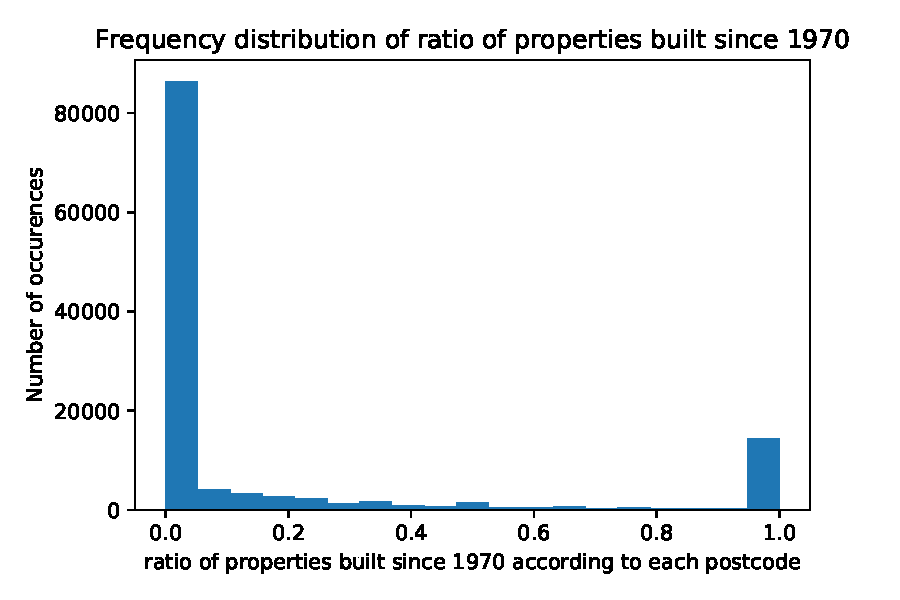
\includegraphics[width=0.6\textwidth]{p9.pdf}
    \end{figure}

For the dataset generated from ‘SW - Lead Comm Pipe Replacements (2004-2018).csv’, our goal is to find the counts of how many times the pipe of each street postcode has been successfully replaced. Also, within the procedure, we could find whether the street has or has not replaced its pipes. To do this, we first read in the dataset an find the information about each feature. Next, we should choose features we need to build a new dataset and make sure all postcodes are capitalized and no blanks in it. Here, we should use the features 'WO Completed Status', 'WO Create Date', and 'Street postcode'. To make sure all the replacement of pipes is valid. We should check the replacement date here to ensure the date of replacement is after 1970. To do this, we need to convert the feature ‘WO Create Date’ to date type, so we can calculate with date type easily. After checking, we find all the samples with dates are after 1970. Then, we check the class types of feature ‘WO Completed Status’.

\begin{figure}[!ht]
    \centering
    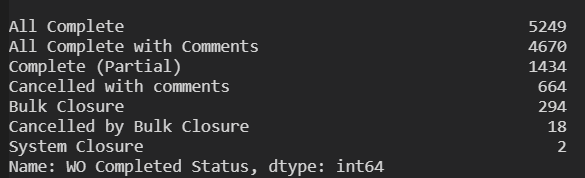
\includegraphics[width=0.6\textwidth]{p10.png}
    \end{figure}

Here we find the classes of this feature for the complete status are mainly two types: ‘All Complete’ and ‘All Complete with Comments’. So, we need to generate a column that records the street postcode with whether its pipe has been finished replacement. we name the new feature as ‘replacement\_finished’. When doing this, we find the elements in ‘WO Completed Status’ have lots of meaningless blanks and we need to delete them before Boolean slicing. And now we can calculate the ratio of the replacement finished, find whether the street has or has not replaced its pipes, and count the number of finished replacements for each street postcode. however, the postcode in the above dataset for Scottish Water is not complete, since this dataset only contains the information of street postcode that may have replaced the pipes. We need to use another dataset called ‘SW - Postcodes linked to SW Zonal Structure’ to find the complete postcode and merge them together. When read in the new dataset we also need to delete the nan value sample points and standardize the postcode format. After let merge, we get a dataset and we need to fill in the NAN values. For the feature ‘any\_replacement’, we replace the NAN value with False. For the feature ‘success\_replacement\_count’, we replace the NAN value with 0. In the below table, we could find that most of the street has not replaced its pipes.

\begin{figure}[!ht]
    \centering
    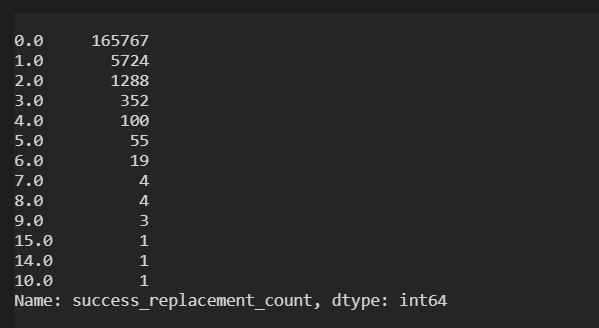
\includegraphics[width=0.6\textwidth]{p11.png}
    \end{figure}

For `SW - All Lead WQ Samples (2010-18)', we first observed that the dataset contains water quality sampling at property level from Scotland. Our goal is to use this dataset to generate an estimation of the water quality (i.e., lead contamination) for each street postcode in Scotland (as long as there is sample for the particular streetcode). So, the most important column in this dataset is clearly `Result Numeric Entry', which records lead concentration in water. The concentration unit column records the unit used for each records. We have checked and assured that for all samples, the unit used are the same (i.e., $\mu$g/l).
In order to obtain an up-to-date estimation of the lead concentration for each area, we wish to use records that are as new as possible. The original sampling has different time periods for different postcodes. For some postcodes, the latest sampling takes place in 2011 or 2012. So it is quite inevitable that our final data would involve records that are quite old (i.e., in year 2011-2012), while some involve newer sampling (e.g., in 2018).

We did not insist on restricting a strict time range for sampling, although that would be ideal for statistical modelling. For example, we didn't require that all sampling must take place in year 2017. The reason is that such restrictions would require us to discard too many samples from our table.
As for each of the records, not all of them have valid sampling result. Some of the results are missing values. The column `Result Status Description' explains why these sampling results are missing. 1241 of these sampling are cancelled. The reason we need to discuss this is that we directly discarded those missing samplings as we believe that cancelling does not have direct relation with lead contamination distribution. We did give one restriction over sampling, that is--for each street postcode, we only keep samples from the last year until the latest sampling. So, for each street postcode, when aggregating the sampling result, we keep at most one year's data. The aim of this is to ensure that the aggregated average lead concentration is as up to date as possible.

For the all Lead WQ sample dataset, we have given a consideration about its statistical robustness as well. We wished to discard postcode data that contain too few sample. However, the majority (16069 samples) of the all the postcodes contained in the dataset corresponds to only a single sample. If we requires that postcodes must contain more than one testing, we would be discarding data related (16069 samples) of all postcodes. Therefore, we consider it better to keep all the sample averages.

The communication pipe dataset `SW - Comm pipe data' is an interesting data set. We have known from an employee of Scottish Water that communication pipes are closely related to lead contamination. We have selected some of the most relevant columns from the dataset including pipe material type, pipe material type at AR10 time, the age of the sampled property, the certainty of the identification of the pipe (as some pipe can be very old and eroded, the identification may not be so accurate), and as the length of the pipe. One interesting varible is `MAIN\_DISTANCE', which estimates the distance of the property from the main pipe. This distance is approximately the distance that the water flows in the communication pipe before it reaches resident's home. It is reasonable conjecture that for especially lead pipes, the longer `MAIN\_DISTANCE' is, the more likely that the water is contaminated.

The detailed operations we did on this dataset are the following. For the identification confidence, as it is a categorical variable but has indeed an ordinal meaning, we convert it directly to numerical values: according to the following table, or we just pick the larger integer in the categorical value.
\begin{center}
    \begin{tabular}{lllc}
        \hline
        categorical confidence  & number of samples & numerical value\\
        \hline
        96-100\%  & 6402   &   100\\
        \hline
        76-95\%   & 4229   &   95\\
        \hline
        51-75\%   &  715   &   75\\
        \hline
        95-100\%  &  474   &   100\\
        \hline
        75-95\%   &  338   &   95\\
        \hline
        50-75\%   &   81   &   75\\
        \hline
        0-50\%    &   24   &   50\\
        \hline
        50-67\%   &    2   &   67\\
        \hline
    \end{tabular}
\end{center}
We did some further reduction on the data. An important information contained in the dataset is the type of the pipe. The origianl column records various types of pipes. For instance: copper, poly, iron, lead, pvc, etc. Since we are going to aggregate the data to postcode level, for sure we can calculate the proportion of pipes for each material, but this would carry a lot of information that is not needed. As our goal is to understand lead contamination, it makes no difference whether a pipe is made of iron or made of PVC. In short, we ultimately only kept the proportion of examined communication pipes that are lead for each postcode. The same is also true for pipe type at ar10.

\subsection{Processed data}
In the final processed data we pull together all the data that we have mentioned above. We left join each of the datasets we mentioned earlier to a base data set which contains all the street postcode in the area. We used the `Trim postcode' column of `SW - Postcodes linked to SW Zonal Structure' as the base dataset. The resulting dataset contains the following colunmns,and we offer a simple data dictionary below:
\begin{center}
    \begin{tabular}{ll}
        \hline
        post\_code                                 &
        street post code\\
        \hline
        rig - PH value                             &
        mean ph value from rig monitor\\
        \hline
        rig - Lead µgPb/l                          &
        mean Lead concentration from rig monitor\\
        \hline
        rig - Phosphorus µgP/l                     &
        mean Phosphorus concentration from rig monitor\\
        \hline
        rig - Temperature °C                       &
        mean Temperature from rig monitor\\
        \hline
        sample - lead µgPb/l                       &
        lead concentration from water quality sample\\
        \hline
        comm pipe - main distance                   &
        average distance from main pip\\
        \hline
        comm pipe - commission year                 &
        average commision year of the communication pipe\\
        \hline
        comm pipe - identification confidence       &
        average confidence of pipe identification\\
        \hline
        comm pipe - leakage                         &
        the ratio of communication pipe discovered leakage\\
        \hline
        comm pipe - property pre 1970               &
        ratio of property before 1970\\
        \hline
        comm pipe - lead pipe ratio                  &
        current ratio of property before 1970\\
        \hline
        comm pipe - ar10 lead pipe ratio             &
        ar10 ratio of property before 1970\\
        \hline
        HPI - Average House Price                  &
        recent average house price based on HPI\\
        \hline
        HPI - Estimated post 1970 ratio            &
        estimated ratio of properties built before 1970\\
        \hline
        replacement - any\_replacement              &
        if any replacement recorded between 2004-2018\\
        \hline
        replacement - success\_replacement\_count    &
        number of communication-pipe replacements 2004-2018\\
        \hline
    \end{tabular}
\end{center}
As is seen in the data dictionary. The naming of the columns first indicates the source of this column before a dash, and appends its detailed name after the dash.

\section{Conclusion}
In this project, we have explored data related to Scottish water lead contamination from several different sources. We have recorded the details of data processings done in order to produce the resulted output data. We have also many whys regarding the decisions we made during the data mergin processes. The resulting data set concentrates the most relevant information related to lead pollution for Scottish Water.

\clearpage

% the entries have to be in the file literature.bib
\bibliographystyle{agsm}
\bibliography{report.bib}
\clearpage

\appendix
\section*{Appendices}
\addcontentsline{toc}{section}{Appendices}

\section{Source Code Link}
\label{app:one}

The git repository of this project is \href{https://github.com/leadPipingProject/leadPiping}{https://github.com/leadPipingProject/leadPiping}.
Please use the \textit{master} branch of the repository.
The python scripts for data cleaning is in folder \href{https://github.com/leadPipingProject/leadPiping/tree/master/code-clean}{code-clean}. It contains the following scripts:

\begin{enumerate}
    \item \href{https://github.com/leadPipingProject/leadPiping/blob/master/code-clean/clean_main.py}{clean\_main.py}: \textbf{this script runs all the scripts below in the right order and merge the results from these scripts into \href{https://github.com/leadPipingProject/leadPiping/blob/master/processed-data/processed_data.csv}{\textit{processed\_data.csv}}. For those who wish to reproduce the data, please run this script.}
    \\
    \textbf{URL: }
    \href{https://github.com/leadPipingProject/leadPiping/blob/master/code-clean/clean_main.py}{https://github.com/leadPipingProject/leadPiping/blob/master/code-clean/\\clean\_main.py}
    \item \href{https://github.com/leadPipingProject/leadPiping/blob/master/code-clean/UK_HPI_clean.py}{UK\_HPI\_clean.py}: this script cleans housing price.
    \\
    \textbf{URL: }
    \href{https://github.com/leadPipingProject/leadPiping/blob/master/code-clean/UK_HPI_clean.py}{https://github.com/leadPipingProject/leadPiping/blob/master/code-clean/\\UK\_HPI\_clean.py}
    \item \href{https://github.com/leadPipingProject/leadPiping/blob/master/code-clean/comm_pipe_clean.py}{comm\_pipe\_clean.py}: this script cleans communication piping data.
    \\
    \textbf{URL: }
    \href{https://github.com/leadPipingProject/leadPiping/blob/master/code-clean/comm_pipe_clean.py}{https://github.com/leadPipingProject/leadPiping/blob/master/code-clean/\\comm\_pipe\_clean.py}
    \item \href{https://github.com/leadPipingProject/leadPiping/blob/master/code-clean/rig_clean.py}{rig\_clean.py}: this script cleans RIG monitor data.
    \\
    \textbf{URL: }
    \href{https://github.com/leadPipingProject/leadPiping/blob/master/code-clean/rig_clean.py}{https://github.com/leadPipingProject/leadPiping/blob/master/code-clean/\\rig\_clean.py}
    \item \href{https://github.com/leadPipingProject/leadPiping/blob/master/code-clean/all_lead_clean.py}{all\_lead\_clean.py}: this script cleans the water quality sampling (2010-2018) data.
    \\
    \textbf{URL: }
    \href{https://github.com/leadPipingProject/leadPiping/blob/master/code-clean/all_lead_clean.py}{https://github.com/leadPipingProject/leadPiping/blob/master/code-clean/\\all\_lead\_clean.py}
    \item \href{https://github.com/leadPipingProject/leadPiping/blob/master/code-clean/pipe_replacement_clean.py}{pipe\_replacement\_clean.py}: this script cleans the communication pipe replacement data.
    \\
    \textbf{URL: }
    \href{https://github.com/leadPipingProject/leadPiping/blob/master/code-clean/pipe_replacement_clean.py}{https://github.com/leadPipingProject/leadPiping/blob/master/code-clean/\\pipe\_replacement\_clean.py/}
    \item \href{https://github.com/leadPipingProject/leadPiping/blob/master/code-clean/property_age_clean.py}{property\_age\_clean.py}: this script cleans the property age data.
    \\
    \textbf{URL: }
    \href{https://github.com/leadPipingProject/leadPiping/blob/master/code-clean/property_age_clean.py}{https://github.com/leadPipingProject/leadPiping/blob/master/code-clean/\\property\_age\_clean.py}
\end{enumerate}

\end{document}
